%Oldaltorest is alkalmazhatunk
% \pagebreak
%laptores:
% \newpage


\documentclass[12pt]{report}
\usepackage[utf8]{inputenc}
%\usepackage[latin2]{inputenc}% ekezetes szavak bevitelehez
\usepackage[T1]{fontenc}
\def\magyarOptions{defaults=hu-min}
\usepackage[magyar]{babel}

\usepackage{times}
\usepackage{tcolorbox}

\usepackage{amsmath}
\usepackage{amssymb}
\usepackage{amsthm}

\usepackage{fancyhdr}

\usepackage{graphicx}
\usepackage{psfrag}

\usepackage{setspace}

\graphicspath{ {./images/} }

%Margok:
\hoffset -1in
\voffset -1in
\oddsidemargin 35mm
\textwidth 150mm
\topmargin 15mm
\headheight 10mm
\headsep 5mm
\textheight 237mm

% \onehalfspacing
\linespread{1.25}

\begin{document}


\thispagestyle{empty}

\begin{center}
{\Large\bf Szegedi Tudományegyetem}

\vspace{0.5cm}

{\Large\bf Informatikai Intézet}

\vspace*{8.5cm}


{\Huge\bf SZAKDOLGOZAT}


\vspace*{7cm}

{\LARGE\bf Marosi Márk Dániel}

\vspace*{0.6cm}

{\Large\bf 2022}

\end{center}

\newpage


\fancypagestyle{plain}{
\fancyhf{}
\fancyfoot[R]{\thepage}
\renewcommand{\headrulewidth}{0pt}
}


\pagestyle{fancy}
\fancyhf{}
\fancyhead[L]{Domain specifikus szöveg feldolgozása kép alapú dokumentumokon}
\fancyfoot[R]{\thepage}


\thispagestyle{empty}

\begin{center}
\vspace*{1cm}
{\Large\bf Szegedi Tudományegyetem}

\vspace{0.5cm}

{\Large\bf Informatikai Intézet}

\vspace*{3.8cm}


{\LARGE\bf Domain specifikus szöveg feldolgozása kép alapú dokumentumokon}


\vspace*{3.5cm}

{\Large Diplomamunka}

\vspace*{4cm}

{\large
\begin{tabular}{c@{\hspace{4cm}}c}
\emph{Készítette:}     &\emph{Témavezető:}\\
\textbf{Marosi Márk Dániel}  &\textbf{Janurik Viktor Bálint}\\
Gazdaságinformatika szakos     &Tanszéki mérnök\\
hallgató&
\end{tabular}
}

\vspace*{2cm}

{\Large
Szeged
\\
\vspace{2mm}
2022
}
\end{center}

\renewcommand{\contentsname}{Tartalomjegyzék}

\chapter*{Feladatkiírás}
\addcontentsline{toc}{section}{Feladatkiírás}

A digitalizáció és az automatizáció terjedésével egyre nagyobb az igény olyan programokra, melyek kép alapú dokumentumokról beolvasott szöveget képesek domain függően feldolgozni és osztályozni predikciók, szövegkörnyezet és a dokumentumon elfoglalt pozíció alapján.\\
A szakdolgozat célja egy ilyen program elkészítése egy tetszőlegesen választott domainnel.


\chapter*{Tartalmi összefoglaló}
\addcontentsline{toc}{section}{Tartalmi összefoglaló}

% \begin{itemize}

    % \item Téma megnevezése:
    % Domain specifikus szöveg feldolgozása kép alapú dokumentumokon

    % \item Feladat megfogalmazása:
    % A szakdolgozat témája és célja az Informatikai Intézet Cisco laborjának távoli elérés rendszerének korszerűsítési keretében történő további két modul fejlesztése.

    % \item A teljes projekt modulokra bontása, munkamegosztás:
    % Egy ilyen projekt túl nagy feladat lett volna egyetlen hallgató számára, éppen ezért a három modult -- web-es frontend, konzolos backend, es az ellenőrző/naplózó köztes modul -- három szakdolgozó fejleszti.

    % \item Alkalmazott módszerek:
    % \begin{itemize}
        % \item Python: A teljes projekt Python nyelven készült, kiegészítve több library-vel: MySQL connector, Pika, Netmiko stb.
        % \item MySQL: a rendszer backend-jéül egy mysql 8.0 szerver szolgál
        % \item RabbitMQ: a komponensek közötti kommunikáció a Rabbit Message Queue segítségével lett megvalósítva
    % \end{itemize}

    % \item Eredmények:
    % A fejlesztés produktuma egy, már alapjaiban működő rendszer, ami további tesztelések, és az ott előjövő problémák javításai után készen áll arra, hogy átvegye a jelenlegi rendszer feladatát.

% \end{itemize}

\tableofcontents

\chapter{Bevezetés}
\addcontentsline{toc}{section}{Bevezetés}
A témaválaszatásomat az informatikai rendszerek elképesztő gyorsaságú fejlődésének gondolata alapozta meg. Egy olyan világban élünk, ahol az okos eszközök elkezdték kiváltani a manuális munkavégzési folyamatokat, vagy azokat egyszerűbbé tették. Minden nap a zsebünkben hordunk egy olyan kompakt eszközt, amely rendelkezik kamerával. Az okostelefonok kamerája, és egy erre fejlesztett applikáció együtt képes kiváltani egy hagyományos szkenner hardvert.

Ezen túlmenve, egyes felsőbb kategóriás telefonok már képesek fényképről felismerni szöveget, és opciót biztosítanak a szöveg kinyerésére is. Amennyiben előttünk van egy névjegykártya, és szeretnénk róla egy nevet vagy telefonszámot gyorsan kimásolni anélkül, hogy nekünk kelljen manuálisan begépelni, egyszerűen készítenünk kell róla egy fényképet, és amennyiben a telefon szöveget talál a képen, azt kimásolhatóvá és vágólapra illeszthetővé teszi a felhasználó számára, ezzel értékes időt spórova, továbbá a hibázás lehetőségét is csökkentve.

Mivel ezek a szoftverek egyre elterjedtebbek, szerettem volna mélyebben belelátni ebbe a témába, viszont egy nemrég történt tapasztalat csak felerősítette szakmai érdeklődésem a szövegfelismerés és feldolgozás kapcsán. 

Egy határátkelésnél történt, hogy a személyi igazolványomat egy kis méterű, kompakt szkennelőgépbe helyezték, és kettő másodperc alatt minden adatom, ami a személyi igazolványomon volt, az a határrendészet szoftverébe került. Ez a folyamat egy olyan plusz lépést tartalmaz az előző, okostelefonos példához képest, hogy itt nem csak az igazolványon található szöveg került felismerésre és beolvasásra, mint egy nagy adathalmaz, hanem a szoftver képes volt ezt az adathalmazt megfelelően szétbontani és osztályozni, felismerte hogy melyik adat a név, melyik adat az állampolgráság, és így tovább.

Szakdolgozatom célja, hogy ezt a témát körbejárjam, felkutassam a legújabb technológiákat és egy ilyen folyamatot be tudjak mutatni egy tetszőlegesen kiválasztott domainnel.
\newline
Ennek megfelelően szakdolgozatomat öt fő részre tagoltam. A dolgozat első részében a jelenleg legismertebb és legmodernebb technológiák utáni kutatásom eredményét fogom részletezni, mélyebben kifejteni azt, hogyan működnek azok a hasonló felhasználási célú redszerek, melyeket jelenleg használnak. A második részben rávilágítok a jelenleg bárki számára elérhető szövegfelismerő rendszerek hiányosságaira, továbbá bemutatom és összehasonlítom azokat a technológiákat, keretrendszereket, amelyeket érdemes lehet felhasználni a projektemben. Harmadik lépésben a projektem megvalósításának részleteit, komponenseit, felépítését fogom bemutatni, valamint megindoklom a domain választásom. Végül lépésről lépésre bemutatom a program működését egy konkrét esetre, valamint a program futásának elvárt eredményét.


% \begin{figure}[h]
    % \centering
    % \includegraphics[scale=0.3]{topology.eps}
    % \caption{A Cisco labor izolált topológiája}
% \end{figure}

\chapter{Jelenlegi rendszerek}
\section{Jelenlegi rendszerek bemutatása}

Egy átlagos felhasználónak kép alapú szövegbeolvasásra jelenleg telefonos vagy web alapú applikációk segítségével van lehetősége. Ez a legegyszerűbb módszer, mert könnyen kezelhető, nem igényel hozzáértést, ingyenesen igénybe vehető, gyors és megbízható. A következőkben egy általam készített, nem valós adatokat tartalmazó minta igazolványon fogom tesztelni az egyik applikációt.

\newline

\begin{figure}[h]
  \centerline{\includegraphics[scale=.25]{example_id_card.eps}}
  \caption{minta igazolvány}
\end{figure}

\pagebreak

A weboldalon található egy fájl feltöltésre alkalmas mező, ide kell tallózni a képet, melyből szeretnénk kinyerni a szöveget, ezután pedig el kell indítani a beolvasási folyamatot, mely körülbelül 5 másodpercet vesz igénybe. A folyamat végén egy szövegmezőből kimásolhatóvá válik a képről kinyert szöveg. Az általam feltöltött képről kinyert szöveg:
\newline
\begin{tcolorbox}
    IDENTIFICATION CARD Family name and Given name: MAROSI MARK DANIEL Sex: MALE Nationality: Date of birth: Date of expiry: Document number: CAN: 123456 HUN 21/09/1999 04/11/2023 123456AB
\end{tcolorbox}
\newline
Az eredményt megvizsgálva megállapítható, hogy a képből kinyert szöveg hibátlan, a betű és a szám alapú adatok is helyesen jelennek meg. Viszont azt is észrevehetjük, hogy az adatok rendezetlenek, nem minden adatról azonosítható be, hogy pontosan mit jelent.

\section{Jelenlegi rendszerek hiányosságai}

Tegyük fel, hogy egy olyan szituációban találjuk magunkat, ahol több személyi igazolványt kell digitalizálnunk, például egy Excel táblázatban eltárolni a kártyán olvasható adatokat. Erre három esetet fogok felvázolni. Az első a klasszikus módszer, ahol közvetlenül a személyi igazolványról írjuk át az adatokat a táblázatba, kézzel begépelve. A második módszer az előbbiekben bemutatott webapplikáció segítségével történne, a harmadik eset pedig egy olyan program használatát feltételezi, melyet a szakdolgozatom keretében fogok elkészíteni.

Amennyiben az első, klasszikus módszert választjuk, kézzel kell beírnunk minden egyes adatot, betűről betűre, számról számra. A három módszer közül ez a leghosszabb és legtöbb emberi hibalehetőséget rejtő módszer. Hibázhatunk az adatok olvasásánál, hibázhatunk az adatok begépelése során, valamint ott is hibázhatunk, hogy nem jó cellába visszük fel az értékeket, elcsúszunk valahol.
\newpage
A második módszer az első módszerben felvázolt három hibalehetőségből kettőt minimálisra csökkent, ezek a beolvasási és begépelési hibák. A beolvasást egy olyan technológiára alapozva végzi a szoftver, amit a szakdolgozat következő fejezeteiben fogok részletesebben bemutatni. Fontos megjegyezni, hogy egyes weboldalak lehetőséget biztosítanak egyszerre akár több kép feltöltésére, ezzel is gyorsítva a folyamatot. A technológia rendkívül pontos, emiatt eltekinthetünk attól, hogy beolvasási hiba történjen, azaz eleve rossz adat kerüljön a táblázatba. A második, begépelési hibalehetőséget kiküszöböli az, hogy a szoftver a beolvasott szöveget másolhatóvá teszi, így szimplán a másolás és beillesztés műveletek segítségével vihetjük fel az adatokat a kívánt cellába. Tehát amennyiben a szövegfelismerés hibátlan volt, úgy minimálisra csökken annak az esélye is, hogy a másolás során elrontsunk valamit. Az egyetlen fennálló hiba továbbra is az, hogy a másolt adatot rossz cellába illesztjük be, összekeverünk két, látszólag hasonló alakiságú adatot, például a születési időt a kártya lejárati dátumával.

A harmadik módszer mind a három hibalehetőségre megoldást biztosítana. A program futása alatt végrehajtott folyamat első része teljes mértékben ugyan úgy történne, mint a második módszer esetében: a feltöltött képről vagy képekről kinyeri a szöveget ugyan azon a technológián alapulva. A program ezután nem a nyers adathalmazt adja vissza a felhasználónak, mint a második esetben, hanem tovább dolgozik azon, és a futás eredménye egy olyan csv vagy excel kiterjesztésű fájl lenne, ahol minden adatkategória (név, állampolgárság, stb.) egy oszlop lenne, és az oszlopnév alatt helyezkedne el a hozzá tartozó adat, például az állampolgárság oszlopban a HUN szöveg. Ezzel teljesen megszűnne minden emberi hibalehetőség, hiszen a teljes folyamatot elvégezné helyettünk a szoftver. Ennek a módszernek további pozitív hozadéka, hogy az adatokat képes az elvárásainknak megfelelően formázni, például a dátumot, amely 30 06 1979 alakot vesz fel a kiolvasás után 1979.06.30 vagy egyéb tetszőleges formára tudná hozni, tovább csökkentve a manuális teendőket.

\chapter{Az OCR technológia}
\section{Az OCR működése}

Az OCR, azaz Optical Character Recognition (magyarul Optikai Karakterfelismerés) egy olyan technológia, amely képes bármilyen képről vagy digitális dokumentumról az írott vagy nyomtatott szöveget felismerni és kinyerni. Az OCR egyik legnagyobb haszna, hogy képes kiváltani a kézi adatbevitelt, jelentős időt spórolva és megszüntetve az emberi hiba lehetőségét is.

\newline
Képzeljünk el egy könyvet, amit egy hagyományos szkennelővel beszkennelünk. A folyamat eredménye digitális képek sorozata lesz, melyeket könnyedén tudunk digitális eszközeink között mozgatni, vagy akár nyomtatóval sokszorosítani tudjuk, de szerkesztni, szöveget keresni vagy kimásolni belőle nem tudnánk. Ha egy olyan szkennerünk lenne, amelyben OCR alapú szövegfelismerés is lenne, akkor a könyvet könnyedén digitalizálhatnánk és nem képeket kapnánk eredményül, hanem egy olyan szöveges dokumentumot, amely teljesen szerkeszthető és kereshető.

\newline
Az Optikai Karakterfelismerés folyamata több lépésből tevődik össze.
Az első lépésben egy osztályozási folyamat történik, ahol a kiválasztott képet vizsgálva a világos területeket háttérnek, a sötét területeket pedig szövegnek minősíti. Ebből kifolyólag az OCR pontosságát tovább javíthatjuk azzal, ha már a karakterfelismerés előtt az inputként választott képet fekete-fehérré alakítjuk.

Második lépésben a szövegként minősített területeken egy olyan keresés indul, amelynek célja az alfabetikus karakterek (betűk) és numerikus karakterek (számok) azonosítása, ez történet karakterről karakterre, vagy szavanként (karakter láncokként) is. Az azonosítás egyik leggyakoribb módszere a mintaillesztésre alapul. Ennél a módszernél egy olyan adathalmazból dolgozik az algoritmus, amely sok különböző betűtípus- és szövegképmintát tárol egy adatbázisban úgy, mint egy sablont. Mikor a képen alakzatot próbál felismerni, összehasonlítást végez a tárolt sablonok alakzatával, és a legnagyobb egyezést mutató karakternek fogja minősíteni a képen látható alakzatot. Ez a módszer akkor igazán pontos, ha az input egy olyan kép, melyen ismert betűtípusokkal jelenik meg gépelt, nyomtatott szöveg, mivel a betűtípusok és kézírási stílusok száma végtelen, és lehetetlen minden típust az adatbázisban rögzíteni. Amennyiben kézzel írt szöveget adunk bemenetként, akkor a pontos eredmény eléréséhez egy olyan algoritmusra van szükség, amely figyelembe veszi a karakterek jellemzőit is. Ilyen jellemzők például a betű írására használt vonalak, azok irányai, elhelyezkedései, metszéspontjai, görbületei és hurkai. Ezen tulajdonságokat az algoritmus minden felismerhető karakterről tárolja, majd a keresett alakzatot is felbontja ugyan ezekre, és megkeresi a tárolt karakterek közül azt, amellyel a legtöbb jellemző megegyezik. Ezt a folyamatot Intelligent Character Recognition (ICR), magyarul Intelligens Karakterfelismerés névvel illetik.

Utolsó lépésben a dokumentum teljes szerekezeti képének függvényében a felismert karakterek önmagukban, szavakba, mondatokba vagy szövegblokkokba rendezve kerülnek tárolásra.

\section{Az OCR pontosságának mérése}

Az előzőekben bemutattam, hogyan képes az OCR egy szöveget tartalmazó képet gépi szöveggé alakítani, de felmerülhet bennünk a kérdés, hogy mégis mennyire pontos az eredmény, amit kapunk egy ilyen konverzió során. A karakterfelismerés csupán képpontról képpontra vizsgálja a képet, és a betűk alakjából vonja le a végső következtetést, arra viszont nem képes, hogy a dokumentum teljes kontextusát felismerve megállapítsa, hogy a szöveg, amit kinyert, az pontosan mit is jelent, és helyesnek bizonyul-e az adott környezetben. Emiatt az OCR gyakran hibázhat, és ezek a hibák pont a szövegfelismerés által adott előnyöket csökkentik.

\newline
Legegyszerűbben úgy határozható meg a pontosság, hogy az OCR kimeneti eredményét összehasonlítjuk a képen szereplő szöveggel. Tegyük fel, hogy a képen szereplő szöveg 100 karakterből áll. Amennyiben az OCR által adott eredményben mind a 100 karakter egyezik az eredeti szövegben szereplővel, akkor azt mondhatjuk, hogy az OCR pontossága 100\%. Amennyiben 99 karaktert sikerült eltalálnia az szövegfelismerőnek, úgy a pontosság 99\%. Tehát egyszerű arányosítással is kiszámolható egyfajta pontosság.

\newline
Most bemutatom a két leggyakrabban használt metrikát, melyek erre a logikára épülnek.

\pagebreak
\subsection{CER - Character Error Rate (Karakter hibaarány)}

A CER mutató azon karakterszintű műveletek minimális számát mutatja meg, amelyek szükségesek a bemeneti szöveg hibátlan kimenetté való konvertálásához.
A CER számításához használt képlet:
\begin{tcolorbox}
    \[CER = \frac{T}{T+C} * 100\]
\end{tcolorbox}
Ahol T az OCR eredményéből érkező karakterek a bemenettel azonos karakterekre való transzformációk számát jelöli (tehát ezek olyan karakterek, melyek helytelenül lettek felismerve), C pedig a helyesen felismert karakterek száma.

\newline
Példa:
\begin{tcolorbox}
    Felismerendő szöveg: abcdefg-123
    \newline
    OCR kimenet: abcdef9-1Z3
    \newline
    Mivel a g betűt 9-es számkarakternek állapította meg, továbbá a 2-es számot Z betűnek, így 2 transzformációra lesz szükségünk, tehát T=2.
    \newline
    A helyesen felismert karakterek száma 9 (a,b,c,d,e,f,-,1,3), ezért C=9.
    \[CER = \frac{2}{2+9} * 100 = 18.18\]
\end{tcolorbox}
Ebben a példában 18\%-os értéket vesz fel a CER mutató, természetesen ez a szám minél kisebb, annál jobb.

\subsection{WER – Word Error Rate (Szóhibaarány)}

Hasonlóan a CER-hez, ennél a metrikánál azt vesszük figyelembe, hogy hány szó szintű műveletre van szükség ahhoz, hogy az OCR folyamat eredménye teljesen megegyezzen a bemeneti szöveggel. Bár a WER érték a szavak metrikáját méri, nem a betűkét, de ha belátjuk, hogy ugyan azon betűk sorozatából kapjuk a szavakat, akkor jogosan feltételezhetjük, hogy a WER és a CER metrikák jól korrelálnak egymással.

\newline
A WER mérésére ugyan azt a képletet használjuk, mint a CER érték méréséhez, de a T paraméter a helyes szóra történő transzformációk számát, a C paraméter pedig nem a helyes karakereket, hanem a teljes terjedelmében helyesen felismert szavak számát jelöli.

\pagebreak
\subsection{További metrikák az OCR pontosságának megállapításához:}

\begin{itemize}
    \item SER - Symbol Error Rate (Szimbólum hibaarány):
    \begin{itemize}
	   \item Ez a metrika kifejezetten azt vizsgálja, hogy a szövegben szereplő szimbólumok, különböző írásjelek milyen arányban kerültek helyesen felismerésre.
    \end{itemize}
    \item Text-Based F1 Score (Szövegalapú F1-pontszám):
    \begin{itemize}
	   \item Ez a mérőszám a felismert szöveg helyes részarányának, illetve a helyesen felismert bemeneti szöveg részarányának a harmonikus átlagát számolja.
    \end{itemize}
    \item Keystroke Saving (Billentyűleütés megtakarítás):
    \begin{itemize}
	   \item Azt méri, hogy ha egy kézi bevitelen alapuló folyamatot egy OCR alapú rendszerrel váltunk ki, akkor hány billentyűleütést spórolunk meg.
    \end{itemize}
\end{itemize}

Fontos megjegyezni, hogy az előbbiekben bemutatott metrikák nem adnak minden esetben valós képet a különböző OCR modellek működéséről, hiszen a beolvasott dokumentumok minősége, valamint a tény, hogy kézírást vagy nyomtatott szöveget adunk bemenetként mind erősen befolyásoló tényezők az OCR kimenetének helyességében.

\section{Az OCR pontosságának javítása bemeneti oldalon}

Az előbbiekben bemutattam, hogyan mérhető az OCR pontossága. Felmerülhet a kérdés, hogy milyen lehetőségek vannak a pontosság javítására. Mivel az OCR egy képről vagy kép alapú dokumentumról hivatott szöveget kinyerni, így a pontos eredmény első és legfontosabb feltétele a megfelelő minőségű bemenet nyújtása. Nézzük, mik azok a leggyakrabban előforduló körülmények, amik rontják az OCR pontosságát.

\begin{itemize}
    \item Az eredeti, szkennelésre váró dokumentum minőségére vonatkozóan:
    \begin{itemize}
        \item Gyűrött, szakadt papír, vagy elmosódott szöveg a papíron
        \item Sérült, lekopott kártya
        \item Fakulás, elszíneződés
        \item Fényes felület
        \item Színes tintával nyomtatott vagy festett szöveg
        \item Nem szokványos betűtípus használata
        \item Emberi kézírás
    \end{itemize}
    \item A beszkennelt vagy kamerával elkészített kép minőségére vonatkozóan:
    \begin{itemize}
        \item Homályos, életlen kép
        \item Elmosódott, torz szélek
        \item Alacsony képfelbontás
        \item Zajosság, szemcsésség
    \end{itemize}
\end{itemize}

Hogy az OCR munkáját elősegítsük, és ezzel javítsuk a pontosságot, az alábbi lépéseket tehetjük, mint felhasználók.

\begin{itemize}
    \item A kép méretének és felbontásának helyes megválasztása:
    \begin{itemize}
	   \item A karakterfelismerés pontossága nagyban függ a bemeneti kép pontsűrűségétől (DPI). 
       \item Általában egy 200-300 közötti DPI-vel rendelkező kép a legmegfelelőbb, ennél kisebb értéknél bizonyos karaktereknél előfordulhat, hogy hibásan kerülnek felismerésre, nagyobb értékeknél pedig szükségtelenül nagy méretű kép lesz a bemenet, az OCR pontossága ezen intervallum felett nem javul számottevően.
    \end{itemize}
    \item Kontraszt növelése és színek eltüntetése:
    \begin{itemize}
	   \item Mivel az OCR egyik lépésre – ahogy azt a működésénél részletesebben kifejtettem –  arra alapul, hogy a képen a világos részeket elválasztja a sötét részektől, és a sötét részeket jelöli meg szövegként, a világos részeket pedig háttérként. Ebből adódik a kép kontrasztjának és színvilágának szerepe a szövegfelismerésben, hiszen a kontraszt minél nagyobb, illetve minél kevesebb szín található a képen, annál pontosabban fogja tudni az OCR leválasztani a szöveget a háttérről.
       \item Az OCR szempontjából egy jó bemeneti kép erősen kontrasztos és csak fekete-fehér színeket tartalmaz. Kontrasztot ma már bármilyen képszerkesztő alkalmazással tudunk növelni, illetve filterek alkalmazásával fekete-fehérré tudjuk alakítani a színes képeket.
    \end{itemize}
    \pagebreak
    \item Ferdeségkorrekció:
    \begin{itemize}
	   \item Amennyiben ferdén fotózott vagy szkennelt képek nagy mértékben csökkentik az OCR hatékonyságát, hiszen a karaktereket meghatározott vonalakból és alakzatokból próbálja felismerni, és ha a képen ferdén vannak a karakterek, akkor nehezebben fog egyezést találni a saját adatbázisában szereplő karakterekkel.
       \item A szkenneléskor vagy fotózáskor törekedni kell arra, hogy a kép minél kevésbé legyen ferde, de lehetőség van utólagos korrekcióra is képszerkesztő program segítségével.
    \end{itemize}
    \item Zajeltávolítás:
    \begin{itemize}
	   \item Törekedni kell arra, hogy a képet megfelelő fényviszonyok mellett készítsük, hogy az minél kevésbé legyen zajos. Bizonyos eljárásokkal csökkenthető az elkészített kép zajossága is simítási, zajmentesítési folyamatokkal, melyek szintén megtalálhatóak a leggyakoribb képszerkesztő programok funkciói között.
    \end{itemize}
\end{itemize}

\chapter{A program megvalósítása}
\section{OCR könyvtárak összehasonlítása Pythonban}

A megvalósítás megkezdése előtt mindenképpen szükséges feltérképezni a rendelkezésre álló OCR könyvtárakat. Ehhez szükséges azt is meghatározni, hogy milyen programozási nyelvben fog a program elkészülni. Hosszas mérlegelés után a Python mellett döntöttem. A Python egy olyan programozási nyelv, amely a népszerűségét többek között a rugalmasságának köszönheti, hiszen a legszélesebb körökben is használható, legyen az webfejlesztés, adatbányászat, gépi tanulás, automatizálás vagy számítógépes grafika. A nyelv továbbá könnyen olvasható egyszerű szintaxisa miatt és támogatja az objektum orientált programozás alapelveit. Népszerűségének alappillére továbbá a folyamatosan fejlődő és bővülő eszközkészlet és a számos ingyenes, nyílt forráskódú könyvtár, melyek a szakdolgozatban is fontos szerepet töltenek be.

A következő alfejezetekben két általam választott ingyenes, nyílt forráskódú OCR könyvtár működését fogom bemutatni, rávilágítva a legfőbb különbségekre.

\subsection{A Pytesseract könyvtár bemutatása}

A Tesseract egy nyílt forráskódú OCR motor, mely számos programozási nyelvvel és keretrendszerrel kompatibilis.
Ahhoz, hogy Pythonból használni tudjuk a Tesseract funkcióit, szükségünk van egy wrapperre, azaz egy olyan könyvtárra, amely python nyelvből teszi lehetővé a Tesseract használatát. A pytesseract nevű könyvtár ezt a célt szolgálja.

\pagebreak

Néhány példa a pytesseract importálása után rendelkezésünkre álló metódusok közül:

Az \textit{image\_to\_string} metódus, ahogy a neve is körülírja, a képről kinyert szöveget egy összefüggő szövegként adja vissza. Ennek a metódushívásnak az eredménye hasonlít leginkább a jelenlegi rendszerek bemutatása fejezetben egy internetes alkalmazás használatával kapott eredményre.

\begin{tcolorbox}
    IDENTIFICATION CARD
    \newline
    Family name and Given name:

    MAROSI MARK DANIEL
    \newline
    sex: MALE Nationality: HUN

    Date of birth: 21/09/1999

    Date of expiry: 21/09/2023

    Document number: 123456AB
    \newline
    CAN: 123456
\end{tcolorbox}

Az \textit{image\_to\_boxes} metódus minden egyes felismert karaktert egyesével, az őt körülhatároló négyzet bal felső sarkának koordinátáival, valamint a négyzet szélességével és magasságával adja vissza listába rendezve.
Egy részlet az eredményhalmazból:

\begin{tcolorbox}
M 3085 2161 3202 2282

A 3213 2161 3334 2282

R 3347 2161 3456 2282

K 3470 2161 3579 2282
\end{tcolorbox}

Az \textit{image\_to\_data} függvény a számunkra leghasznosabb, ugyanis ez figyelembe veszi a karakterek közelségét egymáshoz, ezáltal képes meghatározni szavakat, szorosan összefüggő szövegrészleteket. A szavak mellett visszadja a szót körülhatároló téglalap bal felső sarkának koordinátáját, szélességét, magasságát, valamint azt is, hogy az adott szó vagy szövegrészlet milyen pontossággal került meghatározásra, százalékban kifejezve.
Az, hogy a függvény milyen adatstruktúrában adja vissza a kinyert szavakat, az konfigurálható az output\_type paraméterrel. Választhatunk byte, string, dictionary illetve dataframe opciók közül.

\begin{tcolorbox}
    \begin{center}
        \begin{tabular}{ c c c c c c }
         top & left & width & height & confidence & text \\ 
         956 & 2362 & 653 & 125 & 74 & MAROSI \\  
         958 & 3085 & 494 & 121 & 95 & MARK \\  
         958 & 3638 & 612 & 121 & 95 & DANIEL \\  
        \end{tabular}
    \end{center}
\end{tcolorbox}

\pagebreak
Az \textit{image\_to\_data} függvény eredményének szemléltetése céljából írtam egy függvényt, amely a bemenetként adott igazolványképen a felismert szövegeket határoló téglalapokat kirajzoltattam az OpenCV nevű python könyvtárban definiált metódusok segítségével. Az OpenCV könyvárat a későbbiekben ismertetem. A függvény egy paraméterrel rendelkezik, amely az \textit{image\_to\_data} függvény eredményét várja dictionary struktúrában. A függvény kimenete egy új ablakban megnyíló kép, amelyen a bemeneti kép látható úgy, hogy a rajta található, egyben felismert szövegrészek körül vannak rajzolva a szöveget határoló téglalap élei mentén.

\begin{figure}[h]
    \centerline{\includegraphics[scale=.4]{boxes_pytesseract.eps}}
    \caption{A függvényhívás eredménye, a Pytesseract által kinyert adatok}
\end{figure}

\begin{verbatim}
def generate_image_with_bounding_boxes_on_words(ocr_result):
    img = cv2.imread(ID_CARD_PATH)

    for i in range(len(ocr_result['text'])):
        if float(ocr_result['conf'][i]) >= CONF_LEVEL:
            (x, y, w, h) = (ocr_result['left'][i],
                            ocr_result['top'][i],
                            ocr_result['width'][i],
                            ocr_result['height'][i])
            img = cv2.rectangle(img, (x, y), (x + w, y + h),
                                (0, 255, 0), 10)

    output_img_to_window(img)
\end{verbatim}

\begin{verbatim}
def output_img_to_window(img):
    cv2.namedWindow("output", cv2.WINDOW_NORMAL)
    cv2.imshow("output", img)
    cv2.waitKey(0)
    cv2.destroyAllWindows()
\end{verbatim}

\subsection{Az EasyOCR könyvtár bemutatása}

Az EasyOCR könyvtár is egy nyílt forráskódú, ingyenesen használható OCR könyvtár. A Tesseracttól független, eltérő az implementációja, összességében nagyobb pontosságot képes biztosítani bizonyos esetekben, hátulütője az, hogy nagyobb inputokra lassabb, mint a Tesseract.

Az EasyOCR importálása után először példányosítani kell egy objektumot az easyocr.Reader konstruktorhívással, majd rendelkezésünkre állnak az EasyOCR metódusai. Ezek közül a szakdolgozat szempontjából a \textit{readtext} metódus a legfontosabb, ennek egyetlen paramétere az kép elérési útvonala, melyről szöveget szeretnénk kinyerni.

A metódus egy listával tér vissza, melyben minden listaelem egy szó vagy szövegrészlet, melyet az OCR a karakterek egymáshoz viszonyított pozíciója alapján összefüggőnek ítélt. Minden egyes listaelem további elemeket tartalmaz. Első helyen egy listát, ami az adott szöveget körülvevő téglalap négy sarkának koordináta-párjait tárolja, második helyen magát a felismert szöveget, a harmadik pozíción a pedig tizedestört alakban kifejezve azt, hogy az OCR hány százalékban biztos abban, hogy a kinyert szöveg egyezik a képen látható szöveggel.

\begin{tcolorbox}
    \begin{center}
        \begin{tabular}{ c c c }
         bounding box coordinates & text & confidence \\ 
         {[}{[}329, 78{]}, {[}3551, 78{]}, {[}3551, 350{]}, {[}329, 350{]}{]} & Nationality: & 0.97 \\
        \end{tabular}
    \end{center}
\end{tcolorbox}

Ahogyan azt a pytesseract könyvtár eredményén megtettem, itt is szemléltetésképpen írtam egy metódust, ami a bemenetként adott képen megjeleníti a felismert szavakat, összefüggőnek vélt karakterláncokat.

\pagebreak

\begin{figure}[h]
    \centerline{\includegraphics[scale=.4]{boxes_easyocr.eps}}
    \caption{A függvényhívás eredménye, az EasyOCR által kinyert adatok}
\end{figure}

\begin{verbatim}
def generate_image_with_bounding_boxes_on_words(ocr_result):
    img = cv2.imread(ID_CARD_PATH)

    for text_row in ocr_result:
        bottom_left = tuple(text_row[0][0])
        top_right = tuple(text_row[0][2])
        img = cv2.rectangle(img, bottom_left, top_right, (0, 255, 0), 10)

    cv2.namedWindow("output", cv2.WINDOW_NORMAL)
    cv2.imshow("output", img)
    cv2.waitKey(0)
    cv2.destroyAllWindows()
\end{verbatim}

Ha összehasonlítjuk a két bemutatott könyvtár által adott eredményeket és összevetjük az utóbbi két képet, megfigyelhető, hogy valóban van eltérés a két metódus eredménye között. A legfőbb különbség a szövegrészletek szegmentáltságából adódik: míg az EasyOCR az egymáshoz közel álló szavakat, karakterláncokat sokkal inkább egy egységként dolgozza fel, addig a Pytesseract karakter alapon vizsgálja a dokumentumot, kevésbé érzékeny a kontextusra, ebből adódóan szavakra bontva dolgozza fel a képen olvasható szöveget.

\section{A dokumentum előfeldolgozása}

Ahogyan "Az OCR pontosságának javítása bemeneti oldalon" című fejezetben kifejtettem, a lehető legpontosabb OCR kimenet eléréséhez szükségünk van a bemeneti kép előfeldolgozására pár lépésben az OpenCV nevű ingyenes könyvtár különböző metódusainak használatával.
Mivel a bemeneti dokumentum lehet színes, így először a színek eltüntetésével kezdtem, hiszen a színek a szövegkinyerés szempontjából felesleges információt hordoznak. Ezt az OpenCV cvtColor nevű metódusával értem el, melynek paraméterei egy kép, és az a színtér, melyre konvertálni szeretnénk. A mi esetünkben ez a színtér a COLOR\_RGB2GRAY, ami az RGB színeket a szürke árnyalataivá konvertálja.

\begin{verbatim}
def convert_to_grayscale_image(image):
    return cv2.cvtColor(image, cv2.COLOR_RGB2GRAY)
\end{verbatim}

Következő lépésként a zajeltávolítás volt a célom. Egy zajos kép nagy mértékben ronthatja a kimenet pontosságát, mivel az OCR a zajos, szemcsés részeket is az adott karakter részének határozhatja meg. A zajeltávolítás legegyszerűbb módja a kép kis mértékben történő elmosása, mivel így a zajos részeket összemossuk és jobban beleolvad a háttérbe, cserébe, ha tényleg csak kevés elmosást alkalmaztunk, a karakterek szélei csak kis mértékben veszítenek az élességükből, ezzel továbbra is fenntartva a felismerhetőséget.
Erre a célra a medianBlur metódust hívtam meg az OpenCV könyvtárból, melynek paraméterei a kép és egy 1-nél nagyobb páratlan szám, mely az elmosáshoz használt digitális rekesz lineáris méretét adja meg.

\begin{verbatim}
def remove_noise(image):
    return cv2.medianBlur(image, 5)
\end{verbatim}

Utolsó lépésben a képen található szöveget elkülönítjük a háttértől, amennyire csak lehet. Ezt az OpenCV threshold nevű metódusával érhetjük el, melyet általában arra használnak, hogy egy szürkeárnyalatos képbet kétszintű (bináris) képpé konvertáljanak. A függvény paraméterei a kép, egy küszöbérték (threshold), egy maximum érték (maxval), és a küszöbművelet típusa.
Különböző célokra különböző küszöbműveleti típusok léteznek, számomra a THRESH\_BINARY a legmegfelelőbb.
A THRESH\_BINARY küszöbművelet típus számítási elve:
\begin{equation*}
output(x,y)=
    \begin{cases}
        maxval, & \text{ha}\ input(x,y)>threshold \\
        0, & \text{egyébként}
    \end{cases}
\end{equation*}

A képletből kiolvasható, hogy amennyiben a vizsgált pixel színe a küszöbértéknél nagyobb, akkor a szín átírásra kerül, és a maxvalue értékét fogja felvenni, egyéb esetben az új értéke 0 lesz.
Ahhoz, hogy a szöveg jól elkülönüljön a háttértől, a lehető legszűkebb küszöbértéket kell megadnunk, így a threshold paraméter a mi esetünkben 0 lesz. A maxvalue az a szín, amit a küszöbértéknél nagyobb, azaz kiszűrni kívánt képpontok (ebben az esetben a dokumentum háttere) fog felvenni, ez a mi esetünkben 255 lesz, azaz fehér.

\begin{figure}[h]
    \centerline{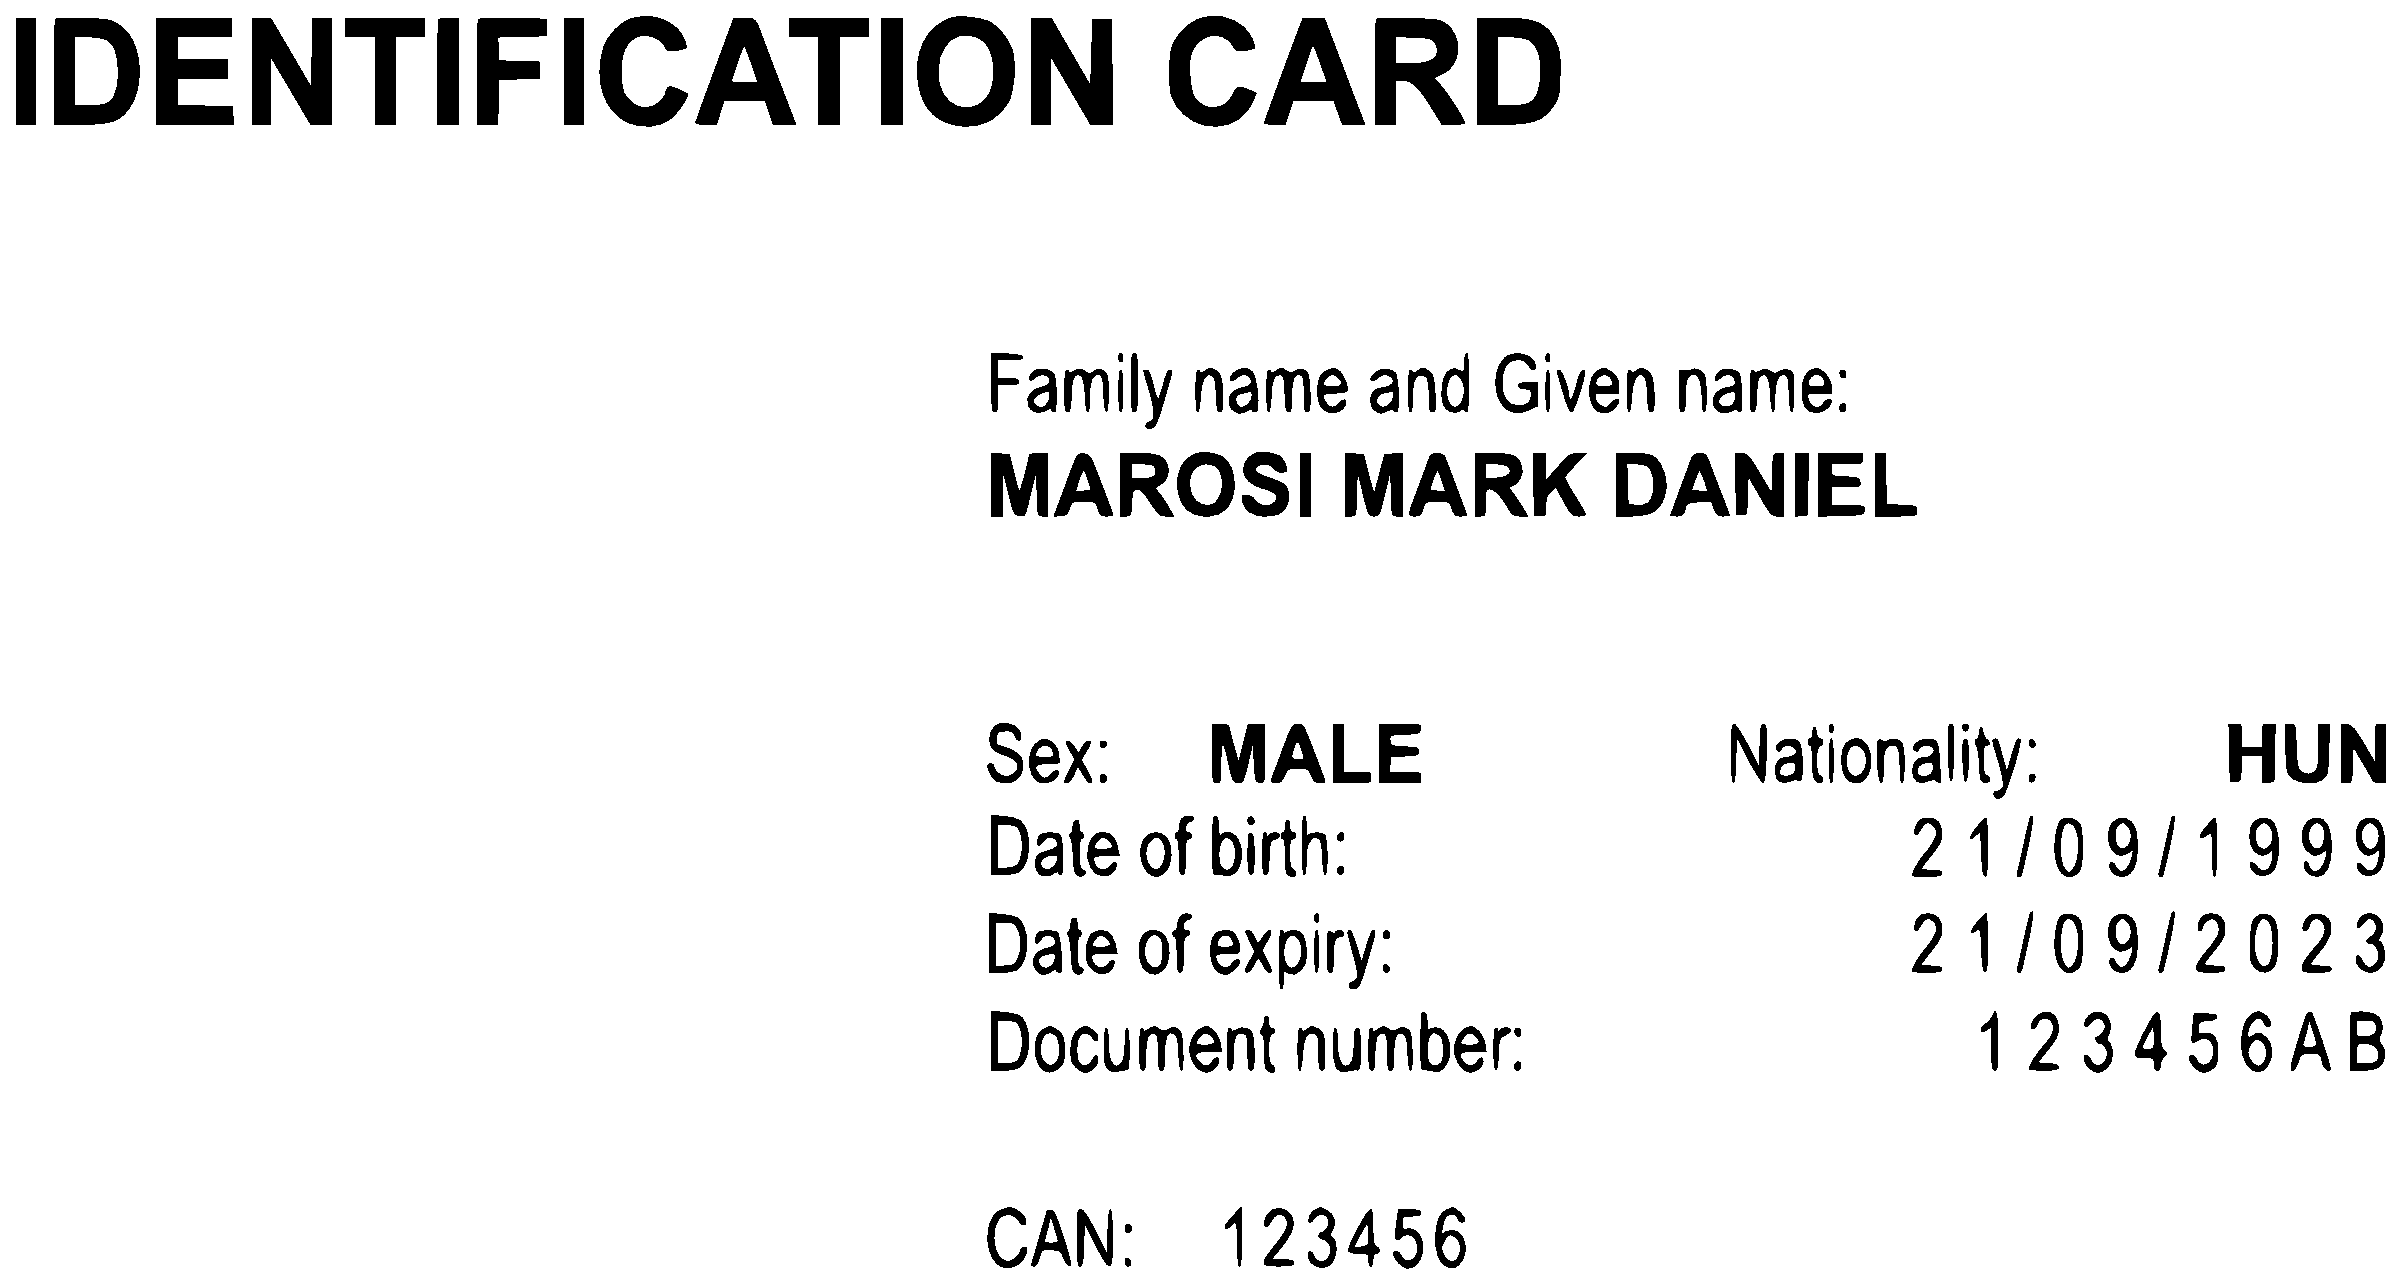
\includegraphics[scale=.25]{preprocessed_image.eps}}
    \caption{A három előfeldolgozó metódus futása utáni állapot}
\end{figure}

\section{Összefoglalás}

A szakdolgozatban leírt projekt lényege, hogy segítséget tudjunk nyújtani a hallgatóknak akár a Cisco hálózatépítő kurzusban, vagy akár a Cisco ipari vizsgára való készülésben. A fejlesztés a szakdolgozaton túl is folytatódik, célunk, hogy egy olyan rendszer álljon a hallgatók rendelkezésére, amivel produktívan lehet tanulni, kísérletezni.


A fejlesztés során lehetőségem nyílt nem csak csapatban, de új technológiákkal is dolgoznom. Köztük a RabbitMQ, aminek használata számomra újdonság és kihívás volt és a Python objektumorientált használata, amire ezelőtt még nem volt szükségem, lehetőségem. Illetve, eddigi tudásomat is lehetőségem nyílt kamatoztatni, a git verziókezelés, a gitlab-runner és a hozzá tarozó CI/CD leírók használata, a docker és docker-compose, és a hyper-v virtualizáció terén.

\chapter{Adatbázis sémák}
%\addcontentsline{toc}{section}{Adatbázis schemák}
\section{Adatbázis sémák}


A program a következő adatbázisokkal dolgozik:

\singlespacing
\begin{itemize}
    \item lab\_tasks
    \item correct\_commands
    \item running\_configs
    \item startup\_configs
\end{itemize}

\onehalfspacing

A lab\_tasks tábla tartalmazza az elérhető feladatok címét, a Cisco tananyag fejezet azonosítóját, amivel a hozzá tartozó tananyag könnyen megtalálható, és COM[1-6] oszlopokat, amelyeknek az értéke a feladat szerinti eszköz hostneve.

A correct\_commands tábla azokat a parancsokat tartalmazza, amelyeket a különböző COM portokon ki kell adni, a feladat helyes elvégzéséhez.

A running\_configs tábla azokat a "show running config" parancs kimeneteket tartalmazza, amelyeket a helyesen konfigurált eszközöknek produkálnia kell.

%\newpage

A startup\_configs tábla pedig a hibaelhárítási feladatokhoz tartozó helytelen beallításokat előállító parancsokat tartalmazza, amelyeket a feladatmegoldás előtt a program futtat az eszközön.

\begin{figure}[h]
    \centering
    \includegraphics[scale=1, angle=90]{table_schema.eps}
    \caption{Séma relációs ábrázolása}
\end{figure}

\chapter{Az alkalmazás működése}
\section{Az alkalmazás működése}


A program belépési pontja a main.py, ami indulásakor példányosítja a MetaCommunication osztályt.
Ez a példány becsatlakozik a RabbitMQ-ba, ahol egy message queue-n figyel, és vár egy felhasználó csatlakozására. A csatlakozást követően készen áll a használatra.

Egy felhasználó csatlakozásakor a MetaCommunication osztály user\_connection() metódusa meghívódik, ezzel példányosítva a User osztályt. A User osztály konstruktora a szükséges adattagokat beállítja (felhaszáló azonosítója, kiválasztott feladat (ha van), helyes parancsok listája, százalékos inkremens).


\begin{figure}[h]
    \centering
    \includegraphics[scale=0.3]{queues.eps}
    \caption{A program indulása előtti és utáni message queue-k}
\end{figure}



A példányosítás után a vezérlés visszatér a MetaCommunication osztály user\_connection() metódusához, ami a Thread típusú User példányt elindítja. Ezzel a User objektum run metódusa meghívásra kerül, ami a programszálat elindítja. Annyi felhasználóhoz tartozó Logger osztálypéldányt készít, ahány COM porton keresztül kommunikál az eszközökkel, továbbá ugyanennyi  QueueListener osztálypéldány is létrejön, ha a felhasználó választott feladatot. Azaz, a jelenlegi felállás szerint egy felhsználóhoz -- a hat COM porthoz -- kétszer hat programszál tartozik, így a MetaCommunication és fő szállal együtt tizennégy vagy nyolc szálon fut a program.

\begin{figure}[h]
    \centering
    \includegraphics[scale=0.3]{threads.eps}
    \caption{A programszálak vizualizálva\\(Készült a PyCharm Concurrent Activities Diagram segítségével)}
\end{figure}

A QueueListener példányok a hozzájuk tartozó message queue-kat figyelik, és az azon keresztül érkező parancsokat fogadják. Feldolgozásra meghívják rájuk a validate\_commands() metódust, ami kiértékeli azt.

%\newpage

Amikor a felhasználó elvégezte a feladatot, a szintjelző 100\%-ra vált, és üzenetet küld a felhasználónak erről.
Ekkor a message queue-kat figyelő szálak feleslegessé válnak, ezért ezeket egyesítjük az őt példányosító szálakkal. 
Ez úgy érhető el, hogy a QueueListener példány is\_waiting\_for\_join tulajdonságát 1-re állítjuk, ami megállítja a futtatását.


A szemétgyűjtést a Python beépített automatikus szemétgyűjtője végzi, ami referenciaszám alapján azokat az objektumokat, amikre már nem hivatkozik semmi, törli a memóriából.
A dokumentációban leírtak alapján a szemétgyűjtés explicit meghívásra kerül, ha az újonnan létrehozott objektumok száma meghaladja a már jelenleg memóriában lévők 25\%-át.
Képletesen felírva:
\begin{equation}
    current\_objects \times 0.25 < new\_objects \Rightarrow garbage\_collection
\end{equation}
Ez a százalékos határ a program esetében ideális. A program indulásakor létrejön a MetaCommunication egy példánya.
Egy felhasználó bejelentkezésekor kétszer hat objektum jön létre (hat QueueListener és hat Logger a hat COM porthoz).
Amikor a felhasználó kijelentkezik, a következő felhasználó bejelentkezéséig két eset állhat fenn.

1. Az automatikus szemétgyűjtés nem fut le, tehát a következő felhasználó bejelentkezésekor az előző felhasználóhoz létrehozott objektumok még a memóriában vanank.

2. Az automatikus szemétgyűjtés lefutott és az előző felhasználó objektumai a következő bejelentkezésekor már nincsenek a memóriában.

Az első eset az, ami vizsgálatot igényel:
Egy felhasználó aktív kapcsolata során 1 + 2 x 6 = 13 objektum van a memóriában, ezek pedig nem törlődtek.
A következő felhasználó bejelentkezésekor 2 x 6 objektum keletkezik. A képletet alkalmazva:
\begin{align*}
    13 \times 0.25 < 12 \\
    3.25 < 12
\end{align*}
Az egyenlőtlenség igaz, tehát a szemétgyűjtés legkésőbb a következő felhasználó bejelentkezésekor meghívódik.


\chapter{Továbbfejlesztési lehetőségek}
%\addcontentsline{toc}{section}{Továbbfejlesztési lehetőségek}
\section{Továbbfejlesztési lehetőségek}

A szakdolgozat keretein belül implementálásra nem került funkcionalitások:
\begin{itemize}
    \item A jelenlegi kód a hálózati erőforrásokhoz (MySQL adatbázis szerver, RabbitMQ) hardcode-oltan csatlakozik, ezért a kód átírása nélkül más fizikiai infrastruktúrára nem lehet telepíteni.
    \item Az adatbázisba leképezett CCNA kurzushoz kapcsolódó laborfeladatok száma igen alacsony, mivel a Word dokumentumokból és PDF fájlokból a konfigurációs lépések kiemelése nem szkriptelhető, ehhez nagy időbefektetés szükséges.
    \item Parancsok kiadása az eszközökön a modul által:
    \begin{itemize}
        \item A felhasználó kijelentkezése után, az eszközök konfigurációjának törlése és az eszközök újraindítása az "indulási konfiguráció" (startup configuration) betöltésével.
        \item A felhasználó által meghívható teljes rendszer visszaállítás arra az esetre, ha valamelyik felhasználó által kiadott parancs elérhetetlenné teszi a rendszert (pl.: jelszó beállításakor félreütött karakter miatti kizárás az eszközről).
    \end{itemize}
    \item A projektben megírt osztályok és metódusaik, mind egy forrásfájlban találhatóak, amely nehezíti a kód olvasását. Ennek több forráskódra bontása, osztályok mentén, ezek csomagokba rendezése és névterek használata, nagyban javítaná a projekt átláthatóságát.
    \newpage
    \item Az idő előrehaladtával a Cisco tananyag verziózásának követése (a jelenlegi rendszer a 6-os verzión alapul). Ez megvalósulhat akár több tábla használatával, vagy akár több adatbázis séma létrehozásával. Ennek megvalósítása biztosítaná, hogy a modul a jövőben ne váljon elavulttá.
\end{itemize}


\begin{thebibliography}{99}
\addcontentsline{toc}{section}{Irodalomjegyzék}

\bibitem{netacad}
Cisco Networking Academy,

v6 \emph{Connecting Networks, Introduction to Networks, Routing and Switching Essentials \& Scaling Networks} Instruktori forrásfájlok


\bibitem{pystruct}
Python projekt struktúrálás és PEP

\emph{https://docs.python-guide.org/writing/structure/}


\bibitem{mysqldoc}
MySQL 8.0 Reference, SQL parancs szintaxisok,

\emph{https://dev.mysql.com/doc/refman/8.0/en/}


\bibitem{mysqlcur}
MySQL Cursor Objects,

\emph{execute és fetch metódusok használata és paramétereik}
\emph{https://mysqlclient.readthedocs.io/user\_guide.html}


\bibitem{docker}
Docker Dokumentáció, parancsok szintaxisa és paramétereik,

\emph{https://docs.docker.com/}


\bibitem{pythread}
Python 3 threading -- Thread-based parallelism,

\emph{https://docs.python.org/3/library/threading.html}


\bibitem{pyobject}
Python 3 Classes,

\emph{https://docs.python.org/3.9/tutorial/classes.html}


\bibitem{mqtt}
MQTT protokoll

\emph{https://mqtt.org/}


\bibitem{rabbitmq}
RabbitMQ Tutorials,

\emph{Work Queues, Publish/Subscribe}
\emph{https://www.rabbitmq.com/getstarted.html}


\bibitem{pika}
Pika AMPQ protokoll implementációs dokumentáció

\emph{https://pika.readthedocs.io/en/stable/}

\end{thebibliography}


\chapter*{Nyilatkozat}
\addtocontents{toc}{\ }
\addcontentsline{toc}{section}{Nyilatkozat}

\noindent
Alulírott Kersmájer István szakos hallgató, kijelentem, hogy a dolgozatomat a Szegedi Tudományegyetem, Informatikai Intézet Szoftverfejlesztési Tanszékén készítettem, gazdaságinformatika diploma megszerzése érdekében.

Kijelentem, hogy a dolgozatot más szakon korábban nem védtem meg, saját munkám eredménye, és csak a hivatkozott forrásokat (szakirodalom, eszközök, stb.) használtam fel.

Tudomásul veszem, hogy szakdolgozatomat / diplomamunkámat a Szegedi Tudományegyetem Informatikai Intézet könyvtárában, a helyben olvasható könyvek között helyezik el.


\vspace*{2cm}


\begin{tabular}{lc}
Szeged, \today\
\hspace{2cm} & \makebox[6cm]{\dotfill} \\
& aláíras \\
\end{tabular}


\chapter*{Köszönetnyilvánítás}
\addcontentsline{toc}{section}{Köszönetnyilvánítás}

Ezúton szeretnék köszönetet mondani Janurik Viktor témavezetőmnek, aki a fejlesztés minden lépésében hasznos tanácsokkal látott el. A segítségéért a tesztkörnyezet összeállításában, a sok konzultációért és szakmai tanácsaiért, amelyek nélkül ez a projekt nem jutott volna tovább az "initial commit"-on.

Köszönöm továbbá két fejlesztőtársamnak, Orbán Veronikának és Csóti Zoltánnak, akikkel a fejlesztés produktívan tudott haladni, és kódváltozásaimhoz igazították saját munkájukat. A hallgatóknak, akik használni fogják az új rendszert, visszajelzéseikért az esetleges problémákról, és további fejlesztési ötleteikért.

\end{document}